\item A manivela $AB$ gira com uma velocidade angular constante de \SI{5}{\radian/\second}. Determine a velocidade do bloco $C$ e a velocidade angular da barra de ligação $BC$ no instante $\theta=30^{\circ}$.

\import{../answers/}{answer-4}

\vspace{-2cm}
\begin{flushright}
	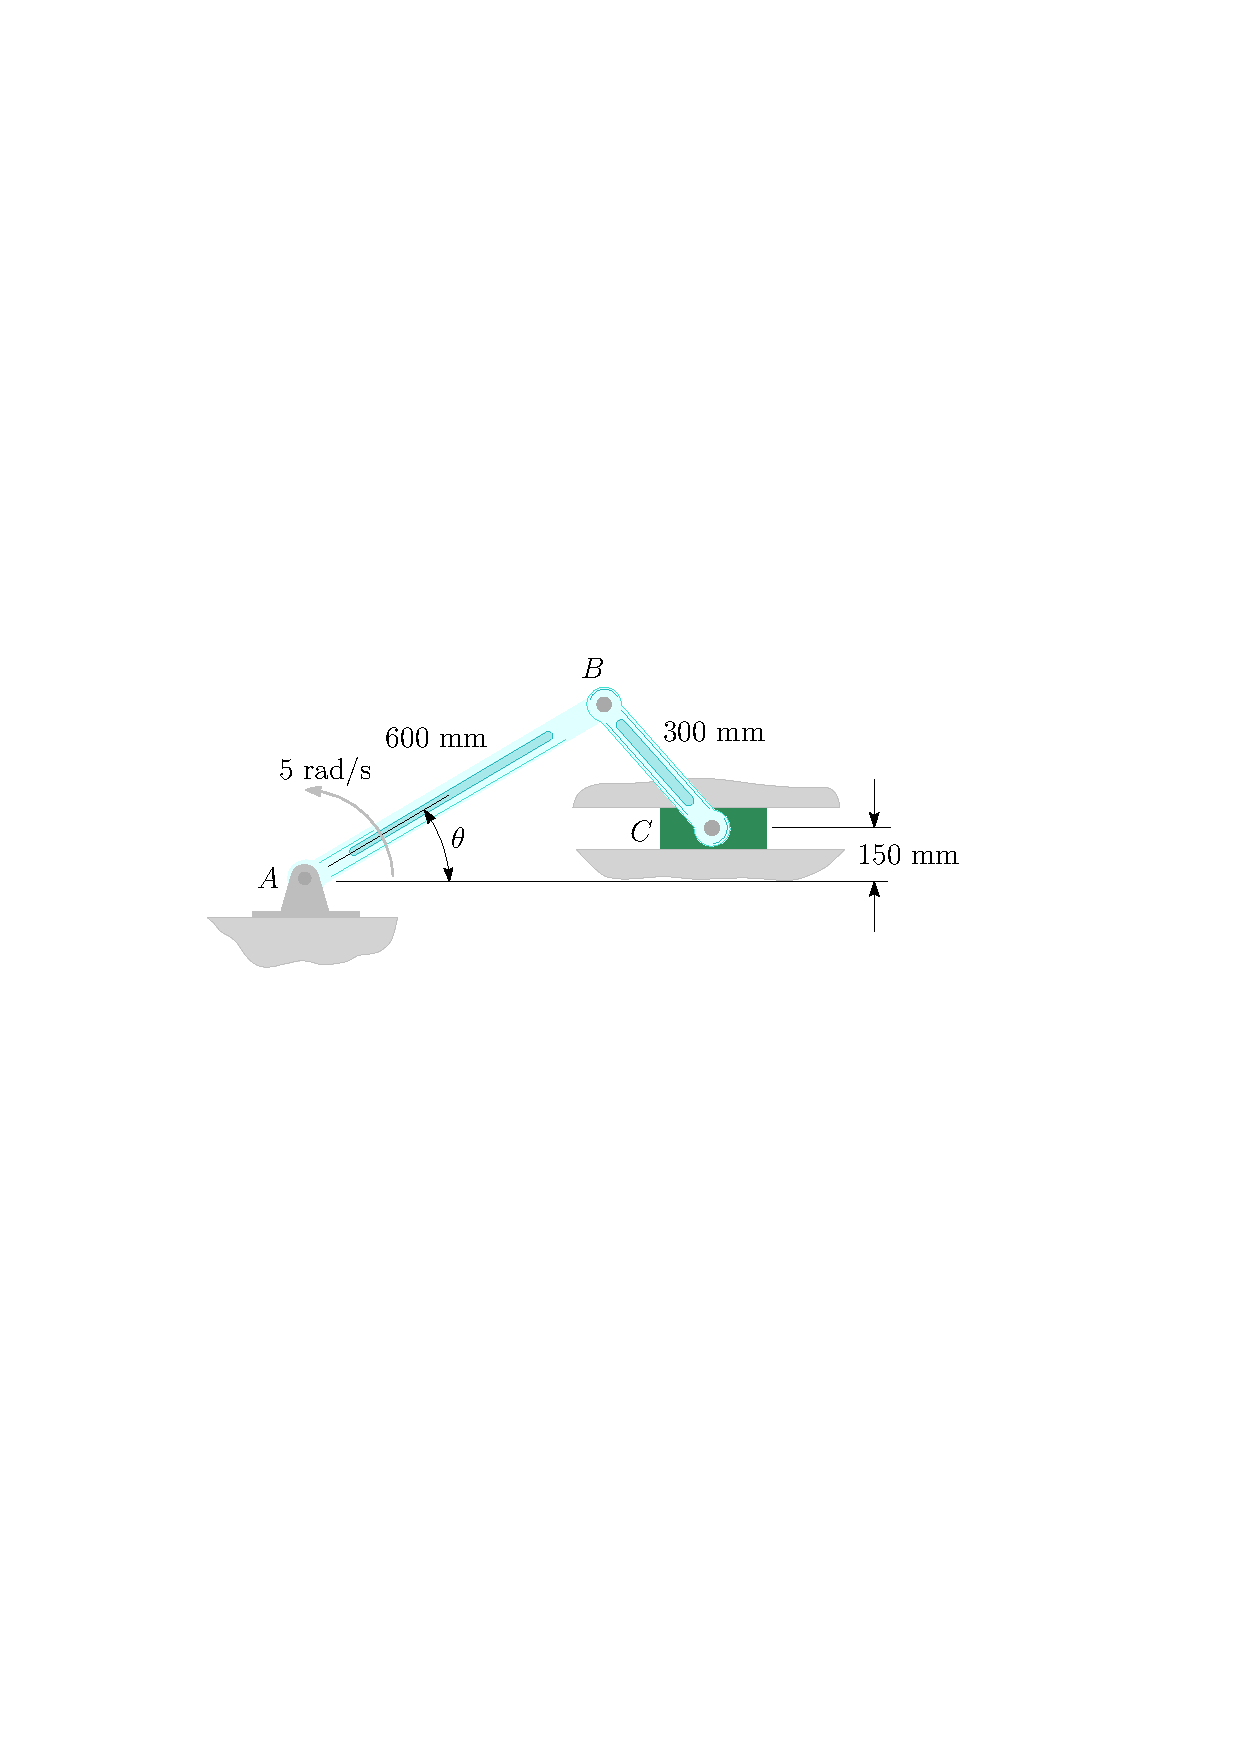
\includegraphics[scale=.9]{images/draw_3}
\end{flushright}